\chapter{Architecture}
\label{ch:architecture}

This chapter presents the architecture of the proposed framework designed to manage uncertainty in SoTS through real-time data reconstruction, confidence propagation, and event reasoning. 

% -------------------------------------------------------------
\section{Architectural Objectives}

The framework architecture is guided by two primary objectives that ensure reliable, interpretable, and interoperable operation across distributed SoTS constituents:

\begin{itemize}
    \item \textbf{Data Continuity:} Preserve uninterrupted information flow within the SoTS by detecting and reconstructing missing data, ensuring that downstream reasoning operates on complete event streams.  

   \item \textbf{Uncertainty Transparency:} Explicitly encode the reliability of reconstructed information as confidence values attached to each event, ensuring consistent handling of uncertainty throughout the processing pipeline.
\end{itemize}

These objectives address a core limitation of existing SoTS and CEP infrastructures, which often assume complete data streams. By integrating reconstruction and confidence tracking directly into the shared event pipeline, the framework replaces absence with approximation. Allowing information to remain accessible even under uncertainty.

% -------------------------------------------------------------
\section{Overview}

The proposed framework adopts a layered, message-driven architecture that enables both autonomy and cooperation among DT constituents within a SoTS. Each DT operates as an independent node capable of reconstructing sensor data, propagating confidence, and performing local event reasoning while remaining connected to a shared asynchronous communication layer.

As shown in Figure~\ref{fig:ch4_context_diagram}, the framework follows a publish subscribe model: each DT publishes data from its own sensors to a shared event stream and may subscribe selectively to datastreams from other constituents. This preserves data ownership while allowing situational awareness to emerge through controlled information exchange. Each DT hosts a local instance of the SoTS framework, configured by a researcher to define subscriptions, reconstruction parameters, and complex event patterns. Through this mechanism, DTs can collaborate and access system-level information without relying on centralized coordination.
\begin{figure}[H]
\centering
\fbox{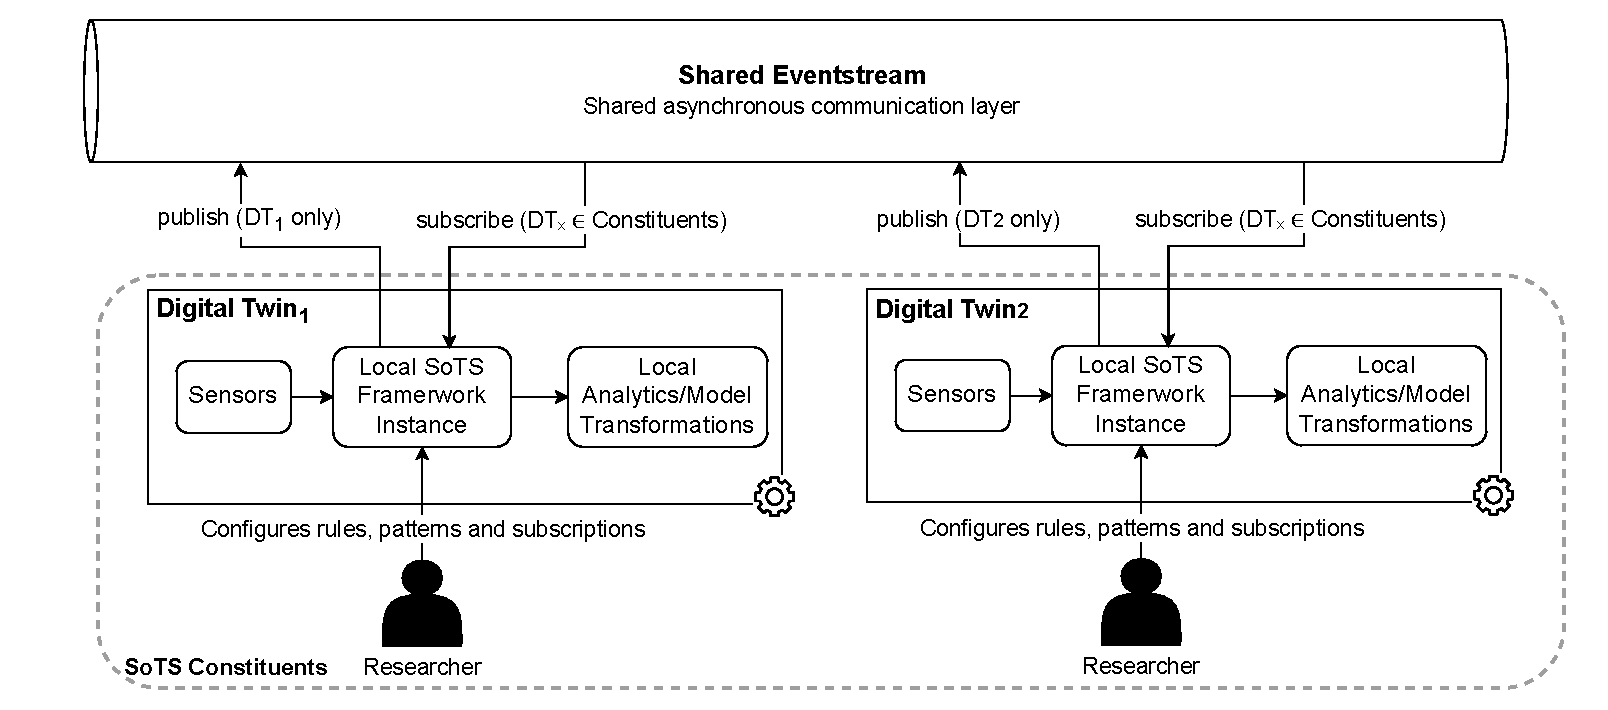
\includegraphics[width=0.95\textwidth]{figures/Architecture/C1 Context.drawio.pdf}}
\caption{Context diagram}
\label{fig:ch4_context_diagram}
\end{figure}

% -------------------------------------------------------------
\subsection{High-Level Pipeline Description}

Figure~\ref{fig:ch4_container_diagram} presents the high-level architecture of the proposed framework. 
The system is organized into two primary layers: the Event Stream Layer, which provides the messaging infrastructure for asynchronous data exchange, and the Processing Layer, which hosts the active modules responsible for coordination, reconstruction, and reasoning. Solid arrows indicate event data flow, while dashed lines represent control signals.

\begin{figure}[H]
\centering
\fbox{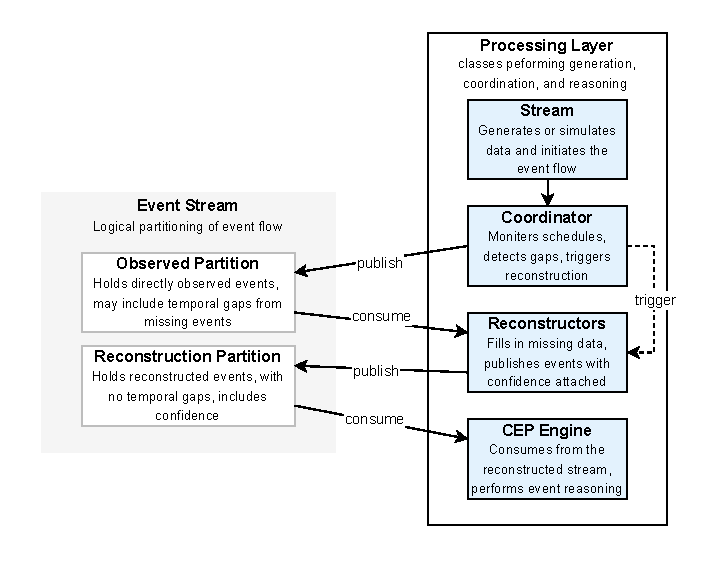
\includegraphics[width=\textwidth]{figures/Architecture/High Level Overview.drawio.pdf}}
\caption{
Container-level Diagram
}
\label{fig:ch4_container_diagram}
\end{figure}

At a high level, the framework operates as a continuous event pipeline that transforms incomplete sensor data into a reconstructed, uncertainty-aware stream. 
\textbf{Streams} act as data generators, emitting observed events that may contain temporal gaps due to missing readings. 
The \textbf{Coordinator} manages event scheduling and serves as the control point for dissemination, publishing available sensor readings to the observed stream or invoking the \textbf{Reconstructor} when expected events are absent. 
The \textit{Reconstructor} consumes all observed data and appends confidence metadata to each event.
It continuously updates the underlying predictors and generates synthetic events when required, producing a unified stream that merges both observed and reconstructed data.
The resulting reconstructed stream provides a temporally complete, confidence-annotated data flow for downstream reasoning by the \textbf{CEP Engine}. 
This design ensures that every event follows a consistent lifecycle from generation to interpretation, maintaining continuity and traceability across the entire pipeline.

\begin{enumerate}
    \item \textbf{Streams} generate sensor data and forward them to the Coordinator.  
    \item The \textbf{Coordinator} schedules event publication, detects missing readings, and triggers reconstruction when gaps are found.  
    \item The \textbf{Reconstructor} consumes observed events, appends confidence information, and imputes missing values when invoked.  
    \item All processed events are published to the \textit{reconstructed stream}, forming a continuous, confidence-annotated data flow.  
    \item The \textbf{CEP Engine} consumes the reconstructed stream for local or global pattern detection.  
\end{enumerate}


% -------------------------------------------------------------
\section{Event Lifecycle and System Flow}\label{sec:system-flow}

\begin{figure}[H]
\centering
\fbox{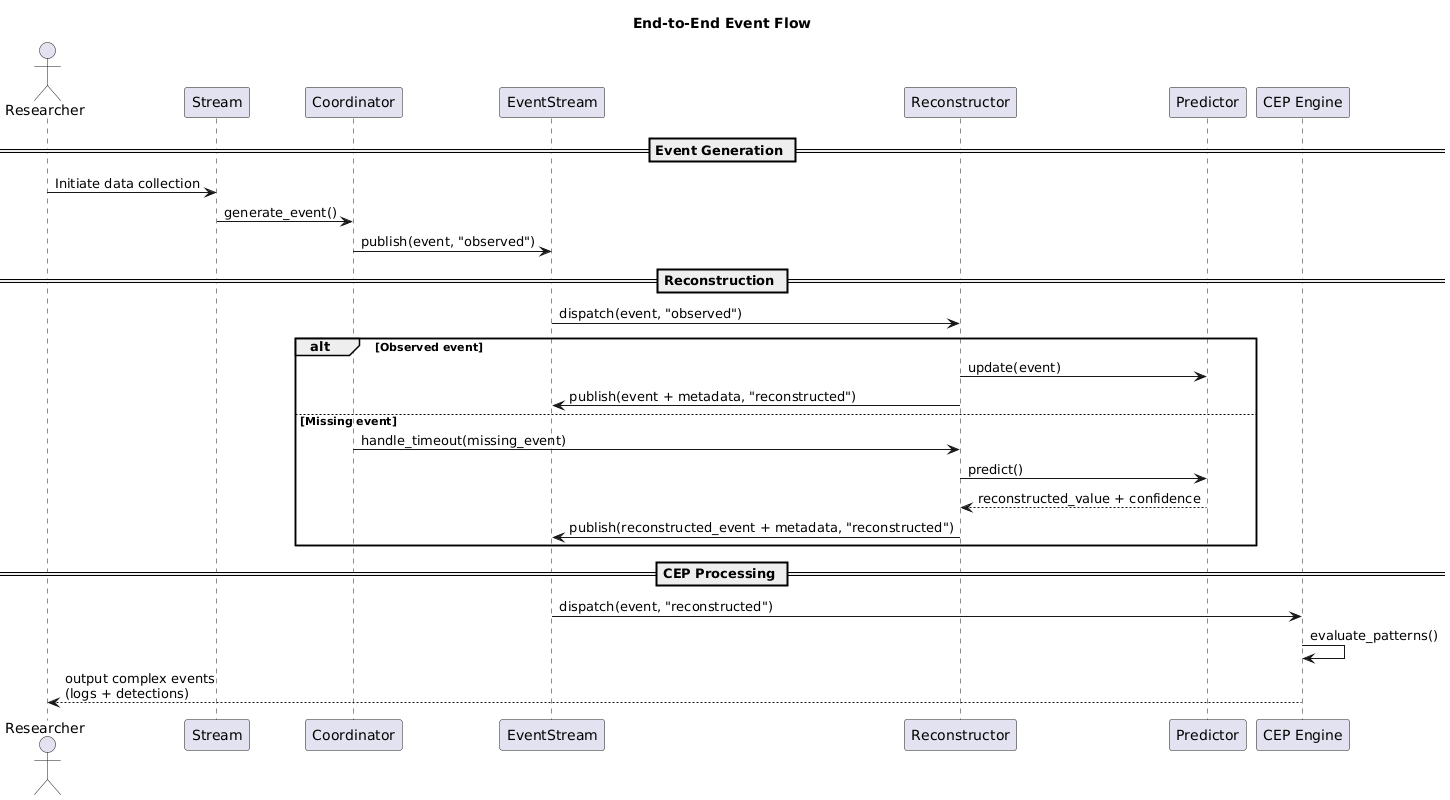
\includegraphics[width=\textwidth]{figures/Architecture/architecture_sequence.png}}
\caption{Flow of an event through the system}
\label{fig:ch4_system_flow}
\end{figure}

The sequence diagram (Figure~\ref{fig:ch4_system_flow}) illustrates the interaction between the major components of the framework.
The process occurs in three phases: \textbf{Event Generation}, \textbf{Reconstruction}, and \textbf{Complex Event Processing}.

\subsubsection*{(1) Event Generation}
The \textit{Researcher} initiates data collection through the \textit{Stream} component.
The \textit{Coordinator} periodically invokes the \texttt{generate\_event()} routine, converting sensor readings into standardized event objects.
Each event is published to the \textit{EventStream} under the \texttt{"observed"} topic, carrying the most recent real sensor values.

\subsubsection*{(2) Reconstruction}
The \textit{Reconstructor} continuously consumes events from the \texttt{"observed"} stream, using the real values to update the internal state of its predictors.
Each event is then augmented with metadata derived from the predictors, such as confidence and the predicted value, and republished into the \texttt{"reconstructed"} stream.
If a temporal gap is detected, the \textit{Coordinator} directly invokes the \textit{Reconstructor}, which synthesizes a missing event using the active predictor (e.g., Kalman filter). The resulting synthetic event is inserted into the reconstructed stream, ensuring that all timestamps are represented and no temporal gaps remain.

\subsubsection*{(3) Complex Event Processing}
The \textit{CEP Engine} subscribes to the \texttt{"reconstructed"} stream and applies pattern-matching rules to detect higher-level phenomena such as anomalies or behavioural trends. 
Each event carries confidence metadata that quantify the estimated reliability of its reconstructed values. 
These attributes are retained throughout the CEP evaluation process, enabling rules to compute, aggregate, and query confidence levels across correlated events. 
The resulting complex events are then logged for downstream analysis.




% -------------------------------------------------------------
\section{UML and Implementation } \label{sec:uml_implementation}

Figure~\ref{fig:architecture_uml} presents the UML diagram of the proposed framework.

\begin{figure}[H]
\centering
\fbox{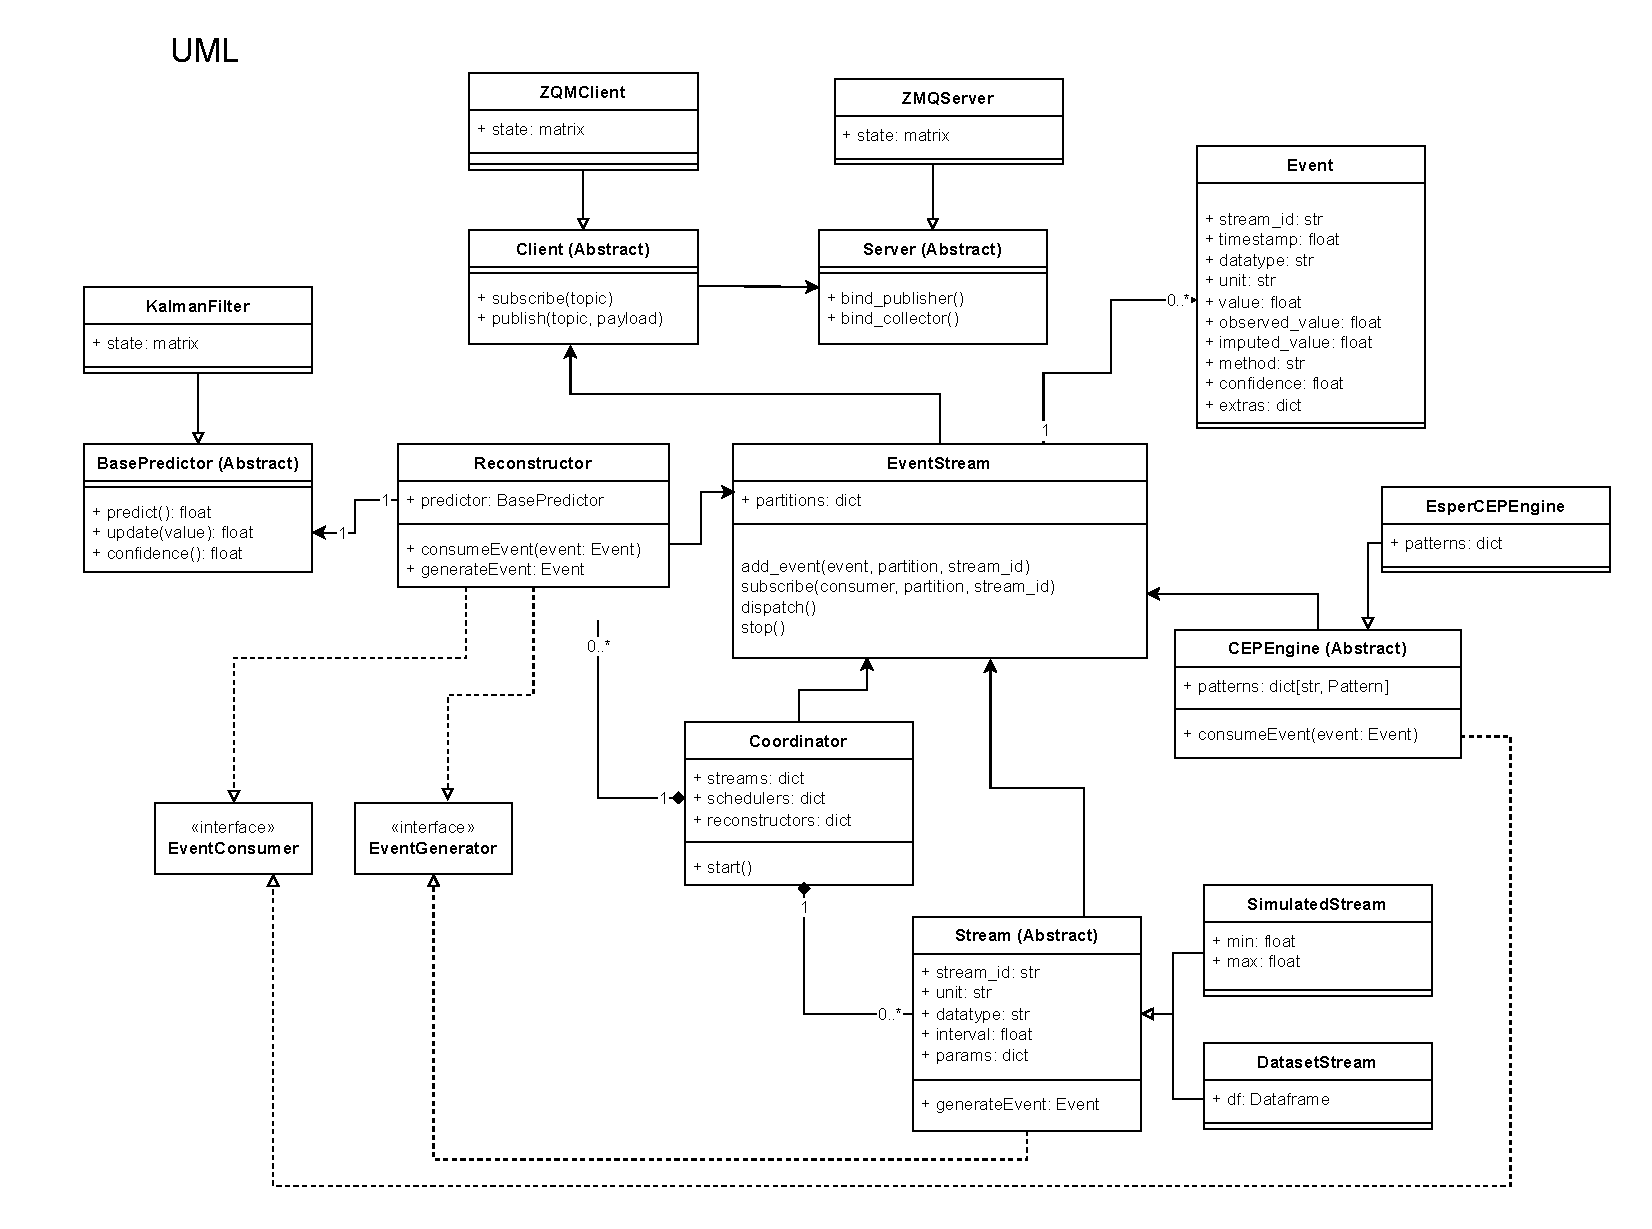
\includegraphics[width=\textwidth]{figures/Architecture/UML.drawio.pdf}}
\caption{UML Class Diagram}
\label{fig:architecture_uml}
\end{figure}
